\documentclass[a4paper,12pt]{article}
\usepackage[utf8]{inputenc}
\usepackage[T1]{fontenc}
\usepackage{graphicx}
\usepackage{hyperref}
\usepackage{listings}
\usepackage{amsmath}
\usepackage{float}
\usepackage{geometry}
\usepackage{polski}

\geometry{margin=1in}

\title{Sprawozdanie z laboratorium 1}
\author{Mikołaj Kubś 272662}
\date{\today}

\begin{document}

\maketitle

\section{Cel zadania}
Celem zadania było zapoznanie się z procesem tworzenia serwerów i stron internetowych za pomocą Node.js oraz Express.js. W późniejszych etapach należało utworzyć obraz Dockerowy, aby zbudować kontener z aplikacją. Ostatecznie należało przekształcić aplikację, aby działała w trybie serverless i wdrożyć ją na jednej z platform chmurowych.

\section{Wykorzystane technologie}
\begin{itemize}
    \item Node.js
    \item Express.js (wraz z Expressjs-layouts)
    \item serverless, serverless-http
    \item Docker - do tworzenia kontenerów
    \item Vercel - do hostowania aplikacji
\end{itemize}

Dodatkowo wszystkie pliki źródłowe zostały napisane w TypeScript, a proces kompilacji został zautomatyzowany przed każdym uruchomieniem aplikacji.

\section{Opis aplikacji}
Aplikacja jest stroną internetową typu Portfolio, która może zawierać informacje o użytkowniku, jego projektach oraz galerię zdjęć. Dotyczy konkretnie autora sprawozdania, jego doświadczenia profesjonalnego i projektach w formie galerii. Dodatkowo aplikacja zawiera formularz kontaktowy, który w przyszłości umożliwi kontakt z autorem.

\section{Opis procesu}
\subsection{Tworzenie aplikacji}
W celu utworzenia aplikacji został stworzony plik o nazwie \texttt{server.ts}, który zawiera kod odpowiedzialny za uruchomienie serwera, konfigurację ścieżek oraz przekierowywanie za pomocą middleware.

Formularz kontaktowy jest obsługiwany przez middleware \texttt{body-parser}, który przekształca dane z formularza na format JSON.

Pliki statyczne, takie jak CSS, skrypty TypeScript czy grafiki, są przechowywane w katalogu \texttt{public}, a ich ścieżka jest przekazywana do middleware \texttt{express.static()}.

\subsection{Dockeryzacja}
Aby utworzyć obraz Dockera, został stworzony plik \texttt{Dockerfile}, który zawiera instrukcje dotyczące budowy obrazu. Następnie za pomocą polecenia:
\begin{lstlisting}[columns=fullflexible]
docker build -t node-web-app .
\end{lstlisting}
został utworzony obraz o nazwie \texttt{node-web-app}. Po zbudowaniu obrazu, można uruchomić kontener za pomocą polecenia:
\begin{lstlisting}[columns=fullflexible]
docker run -p 4000:4000 -d node-web-app
\end{lstlisting}

\begin{figure}[H]
    \centering
    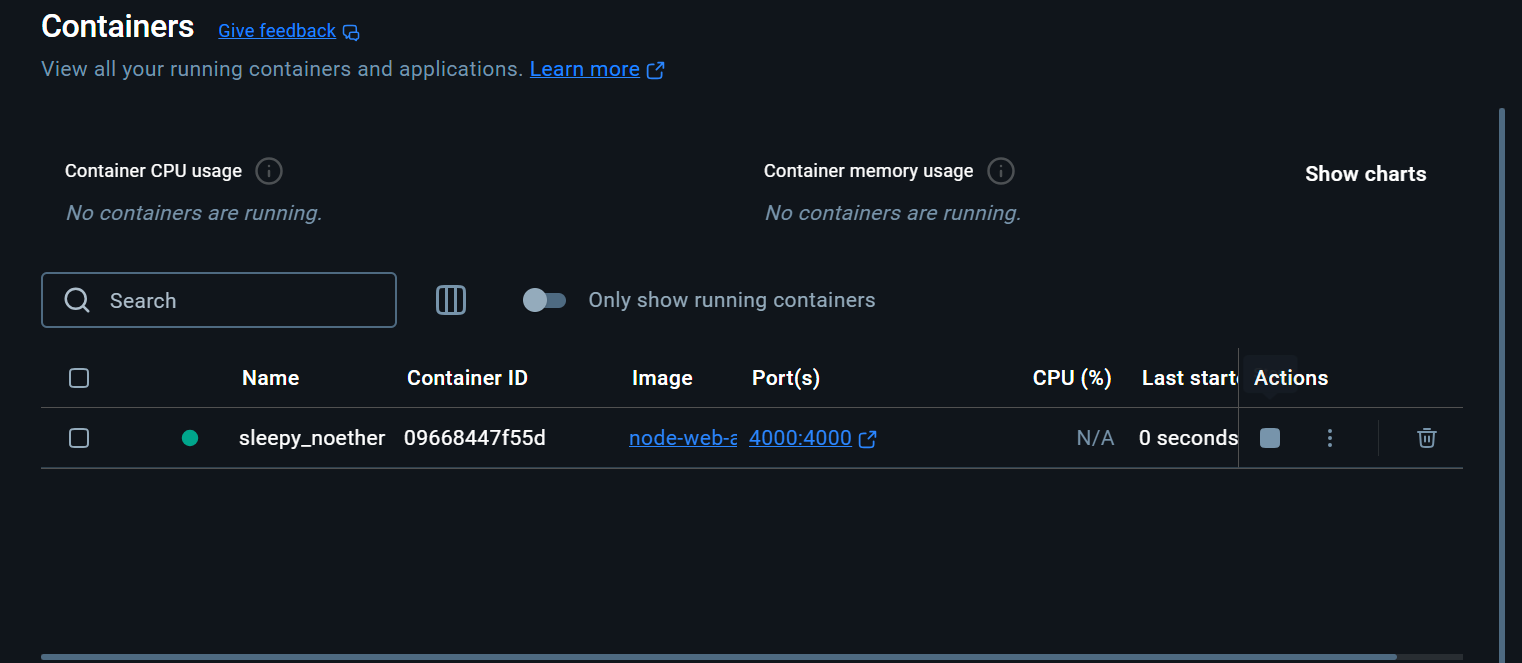
\includegraphics[width=1\textwidth]{images/docker.png}
    \caption{Kontener załadowany w Docker Desktop}
\end{figure}

\subsection{Serverless}
Aby przekształcić aplikację w tryb serverless, zostały wykorzystane dwie biblioteki: \texttt{serverless} oraz \texttt{serverless-http}. Następnie zmodyfikowano kod w pliku \texttt{server.ts} oraz dodano plik konfiguracyjny \texttt{serverless.yml}.

Za pomocą polecenia:
\begin{lstlisting}[columns=fullflexible]
serverless start-offline
\end{lstlisting}
można uruchomić aplikację w trybie offline, co pozwala na testowanie aplikacji bez potrzeby wdrażania jej na platformę chmurową. Problemem, który napotkałem podczas uruchamiania aplikacji w trybie offline, był brak dostępu do plików statycznych, tj. obrazów. Pozostałe pliki typu \texttt{js} oraz \texttt{css} w folderze \texttt{public} były dostępne. Mimo że pliki z obrazami były poprawnie przekazywane, to nie były wyświetlane. Żeby naprawić ten problem, trzeba było poprawić plik \texttt{serverless.yml}, dodając odpowiednie include'y i akceptowalne typy binarne mediów.

\subsection{Wdrożenie aplikacji na Vercel}
Aby wdrożyć aplikację na Vercel, należy zainstalować CLI Vercel oraz utworzyć konto na platformie. Następnie należy zalogować się do swojego konta za pomocą polecenia:
\begin{lstlisting}[columns=fullflexible]
vercel login
\end{lstlisting}
Po zalogowaniu się można wdrożyć aplikację za pomocą polecenia:
\begin{lstlisting}[columns=fullflexible]
vercel
\end{lstlisting}
Oraz deployować na produkcję:
\begin{lstlisting}[columns=fullflexible]
vercel --prod
\end{lstlisting}
Oraz testować vercel lokalnie:
\begin{lstlisting}[columns=fullflexible]
vercel dev
\end{lstlisting}
Strona znajduje się pod linkiem: \href{https://web-app-five-dusky.vercel.app/}{Portfolio Mikołaj Kubś}.

Wdrożenie aplikacji przebiegło względnie bezproblemowo. Wystąpiły problemy z ładowaniem treści strony, a potem obrazów czy plików JavaScript. Należało poprawić \texttt{vercel.json}, \texttt{tsconfig.json} oraz \texttt{server.ts}. Część błędów powstała przez używanie TypeScript i kompilacji plików do folderu \texttt{dist}.

\section{Wygląd aplikacji}

\begin{figure}[H]
    \centering
    
\includegraphics[width=1\textwidth]{images/page_top.png}
    \caption{Wygląd strony}
\end{figure}

\begin{figure}[H]
    \centering
    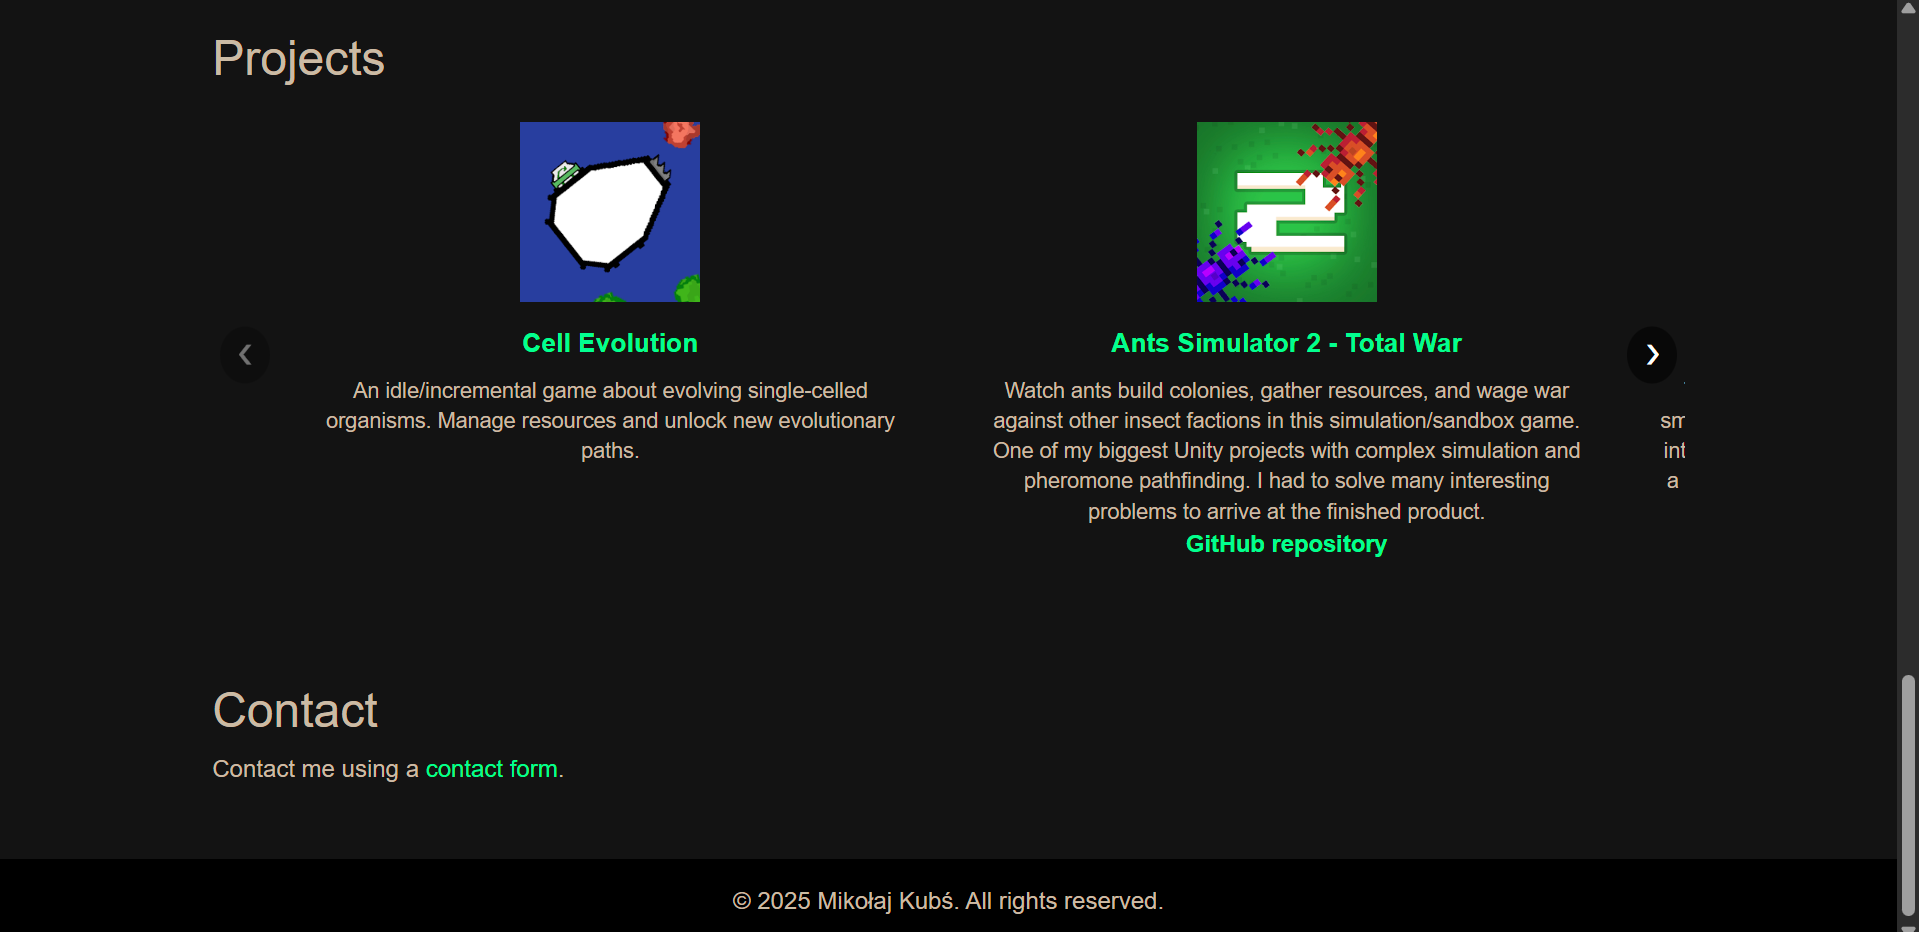
\includegraphics[width=1\textwidth]{images/gallery.png}
    \caption{Wygląd galerii z projektami}
\end{figure}

\begin{figure}[H]
    \centering
    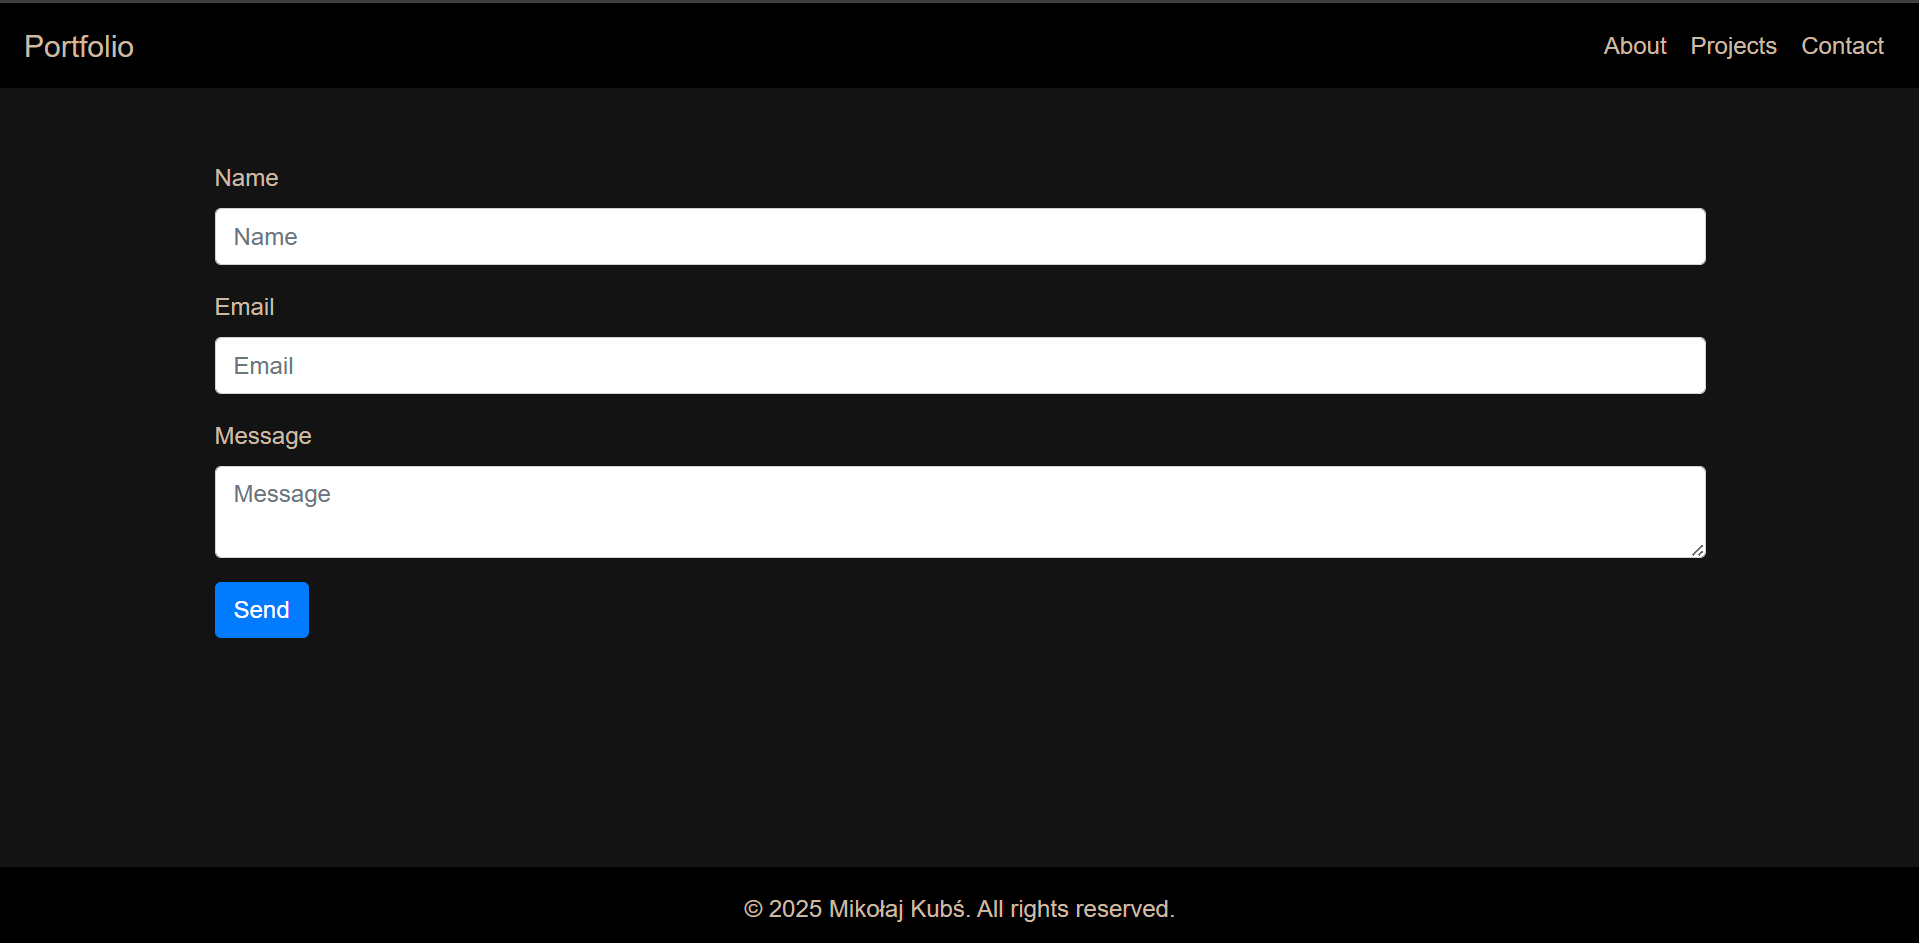
\includegraphics[width=1\textwidth]{images/contact.png}
    \caption{Wygląd formularza z kontaktem}
\end{figure}

\end{document}
